% Guardrails Before the Fall: Anticipatory Governance for AI, Quantum, and Neuromorphic Systems
% Author: Clarence H. Cannon, IV
% File: paper/main.tex

\documentclass[11pt,twocolumn]{article}
\usepackage[utf8]{inputenc}
\usepackage[T1]{fontenc}
\usepackage{geometry}
\usepackage{hyperref}
\usepackage{graphicx}
\usepackage{booktabs}
\usepackage{amsmath}
\usepackage{natbib}
\usepackage{xcolor}
\usepackage{float}
\usepackage{tikz}
\usetikzlibrary{positioning,arrows.meta,shapes.geometric,calc,backgrounds,fit,decorations.pathreplacing}

\geometry{margin=1in}
\hypersetup{colorlinks=true,linkcolor=blue,citecolor=blue,urlcolor=blue}

\title{\textbf{Guardrails Before the Fall: Anticipatory Governance for AI, Quantum, and Neuromorphic Systems}}

\author{
Clarence H. Cannon, IV\\[0.5em]
\small University of Colorado Boulder\\
\small Boulder, CO\\[0.5em]
\small \texttt{Clarence.Cannon@colorado.edu}
}

\date{November 2025}

\begin{document}

\maketitle

\begin{abstract}
Frontier artificial intelligence, neuromorphic computing, and quantum systems are converging on accelerated timelines, presenting unprecedented governance challenges. Current containment strategies---particularly red-teaming---while necessary, are demonstrably insufficient as standalone control mechanisms. This paper argues that anticipatory governance frameworks must be established \textit{before} potential market corrections in the AI sector, not after. Drawing on empirical jailbreak studies, responsible scaling policies, and emerging regulatory frameworks (EU AI Act, US Executive Order 14110), we propose a multi-layered governance architecture that binds safety measures to scaling thresholds, deployment contexts, and cross-domain coupling. We present minimal-compute experiments demonstrating persistent model vulnerabilities and propose policy interventions that balance innovation enablement with meaningful risk mitigation. The core thesis: guardrails implemented during periods of growth are more robust than those hastily constructed amid market instability.
\end{abstract}

\textbf{Keywords:} AI governance, responsible scaling, red-teaming, neuromorphic computing, quantum supremacy, anticipatory regulation, AI safety

%==============================================================================
\section{Introduction}
%==============================================================================

The artificial intelligence sector is experiencing unprecedented capital inflows and capability advances. However, as with previous technology cycles, questions arise about sustainability and the consequences of potential market corrections. Central banks and financial institutions have noted AI-driven bubble dynamics \cite{apnews2024bubble}, while industry leaders acknowledge a ``kernel of truth amid hype'' \cite{verge2024altman}.

This paper argues that governance frameworks must be anticipatory rather than reactive. The conventional wisdom---``don't regulate during growth''---inverts the prudent approach. Market corrections do not eliminate risk; they may amplify it as firms cut safety investments and race to demonstrate viability. Guardrails established during stability are more robust than those constructed amid instability.

Three converging technological frontiers compound the urgency:

\begin{enumerate}
    \item \textbf{Frontier AI}: Large language models and agentic systems with expanding tool-use capabilities
    \item \textbf{Neuromorphic Computing}: Brain-inspired architectures achieving energy efficiencies that democratize compute access
    \item \textbf{Quantum Systems}: Advancing toward practical advantage in optimization and cryptographic domains
\end{enumerate}

Each frontier presents distinct governance challenges. Their convergence---neuromorphic systems running AI workloads, quantum-enhanced optimization of neural architectures---creates risk surfaces that current frameworks do not adequately address.

%==============================================================================
\section{State of Play: Current Regulatory Landscape}
%==============================================================================

\subsection{Regulatory Timeline}

Figure~\ref{fig:timeline} illustrates the staggered implementation of major regulatory frameworks against projected capability milestones.

\begin{figure*}[t]
\centering
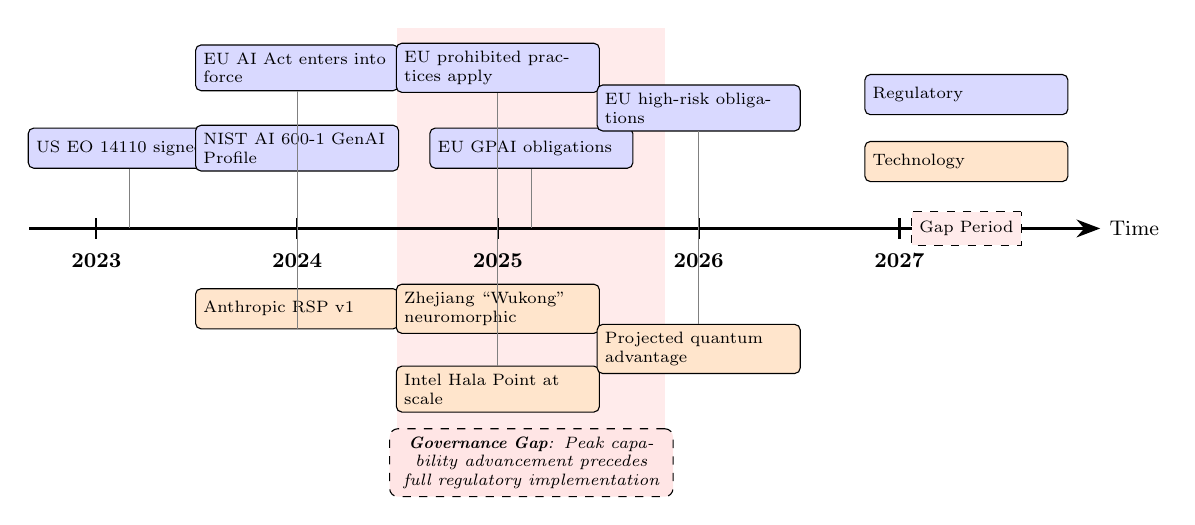
\begin{tikzpicture}[
    scale=0.85,
    transform shape,
    yearnode/.style={font=\bfseries\small, text=black},
    regnode/.style={draw, rounded corners=2pt, fill=blue!15, font=\scriptsize, text width=2.8cm, align=left, minimum height=0.6cm},
    technode/.style={draw, rounded corners=2pt, fill=orange!20, font=\scriptsize, text width=2.8cm, align=left, minimum height=0.6cm},
    gapnode/.style={draw, dashed, rounded corners=3pt, fill=red!10, font=\scriptsize\itshape, text width=4cm, align=center},
    arrow/.style={-{Stealth[length=2mm]}, thick, gray}
]

% Main timeline axis
\draw[very thick, -{Stealth[length=3mm]}] (0,0) -- (16,0) node[right, font=\small] {Time};

% Year markers
\foreach \x/\year in {1/2023, 4/2024, 7/2025, 10/2026, 13/2027} {
    \draw[thick] (\x,0.15) -- (\x,-0.15);
    \node[yearnode, below] at (\x,-0.25) {\year};
}

% Regulatory events (above timeline - blue)
\node[regnode] (eo) at (1.5,1.2) {US EO 14110 signed};
\node[regnode] (euforce) at (4,2.4) {EU AI Act enters into force};
\node[regnode] (nist) at (4,1.2) {NIST AI 600-1 GenAI Profile};
\node[regnode] (euproh) at (7,2.4) {EU prohibited practices apply};
\node[regnode] (eugpai) at (7.5,1.2) {EU GPAI obligations};
\node[regnode] (euhigh) at (10,1.8) {EU high-risk obligations};

% Technology events (below timeline - orange)
\node[technode] (rsp) at (4,-1.2) {Anthropic RSP v1};
\node[technode] (wukong) at (7,-1.2) {Zhejiang ``Wukong'' neuromorphic};
\node[technode] (hala) at (7,-2.4) {Intel Hala Point at scale};
\node[technode] (quantum) at (10,-1.8) {Projected quantum advantage};

% Connecting lines to timeline
\foreach \node in {eo, nist, rsp} {
    \draw[gray, thin] (\node.south) -- (\node.south |- 0,0);
}
\draw[gray, thin] (euforce.south) -- (euforce.south |- 0,0);
\draw[gray, thin] (euproh.south) -- (euproh.south |- 0,0);
\draw[gray, thin] (eugpai.south) -- (eugpai.south |- 0,0);
\draw[gray, thin] (euhigh.south) -- (euhigh.south |- 0,0);
\draw[gray, thin] (wukong.north) -- (wukong.north |- 0,0);
\draw[gray, thin] (hala.north) -- (hala.north |- 0,0);
\draw[gray, thin] (quantum.north) -- (quantum.north |- 0,0);

% Governance gap shading
\begin{scope}[on background layer]
    \fill[red!8] (5.5,-3) rectangle (9.5,3);
\end{scope}

% Gap annotation
\node[gapnode] at (7.5,-3.5) {\textbf{Governance Gap}: Peak capability advancement precedes full regulatory implementation};

% Legend
\node[regnode, minimum width=1.5cm] at (14,2) {Regulatory};
\node[technode, minimum width=1.5cm] at (14,1) {Technology};
\node[draw, dashed, fill=red!8, minimum width=1.5cm, minimum height=0.5cm, font=\scriptsize] at (14,0) {Gap Period};

\end{tikzpicture}
\caption{Timeline of regulatory milestones and technology developments (2023--2027). The shaded region indicates the governance gap where peak capability advancement (2024--2025) precedes full regulatory implementation (2026+). Blue boxes represent regulatory events; orange boxes represent technology milestones.}
\label{fig:timeline}
\end{figure*}

\subsection{European Union AI Act}

The EU AI Act, enacted in 2024, represents the most comprehensive AI regulatory framework to date. Key provisions phase in through 2026, with general-purpose AI (GPAI) obligations taking effect earlier \cite{euaiact2024}. The Act establishes:

\begin{itemize}
    \item Risk-based classification (unacceptable, high, limited, minimal risk)
    \item Transparency requirements for GPAI models
    \item Mandatory conformity assessments for high-risk systems
    \item Incident reporting and post-market monitoring obligations
\end{itemize}

However, implementation timelines create regulatory gaps during precisely the period of most rapid capability advancement.

\subsection{United States Executive Order 14110}

Executive Order 14110 (October 30, 2023) directs federal agencies to develop AI safety standards, reporting requirements, and evaluation frameworks \cite{eo14110}. Key directives include:

\begin{itemize}
    \item NIST development of AI Risk Management Framework guidance
    \item Reporting thresholds for large training runs
    \item Content provenance and watermarking standards
    \item Dual-use foundation model evaluation requirements
\end{itemize}

The NIST AI Risk Management Framework 1.0 and subsequent Generative AI Profile (NIST-AI-600-1, July 2024) provide concrete implementation guidance \cite{nistrmf, nistgenai}.

\subsection{International Coordination}

The UK AI Safety Institute has conducted joint pre-deployment evaluations with US counterparts, finding persistent vulnerabilities including ``easy jailbreaks across frontier models'' \cite{aisi2024, guardian2024jailbreak}. The International AI Safety Report synthesizes global capability and risk trajectories \cite{internationalsafety}.

%==============================================================================
\section{Are Current Controls Sufficient? The Red-Teaming Question}
%==============================================================================

\subsection{What Red-Teaming Provides}

Red-teaming---adversarial testing to identify model vulnerabilities---has become the default safety intervention. The NIST Generative AI Profile specifies red-teaming as a component of Testing, Evaluation, Verification, and Validation (TEVV) \cite{nistgenai}. CISA positions red-teaming within broader TEVV pipelines \cite{cisa2024}.

Industry implementations vary. OpenAI's external red-teaming process engages domain experts for pre-deployment testing \cite{openai2024redteam}. Anthropic's Responsible Scaling Policy (RSP) ties capability thresholds to safety requirements, including red-team evaluations \cite{anthropicrsp}.

\subsection{What Red-Teaming Does Not Provide}

Critical scholarship identifies fundamental limitations. Feffer et al. (2025) document ``scope creep and gaps'' in red-teaming practices, noting that the term encompasses heterogeneous activities with inconsistent standards \cite{arxiv2025redteam}. CSET recommendations emphasize the need to ``strengthen AI red-teaming'' through standardization and independence requirements \cite{cset2024}.

UK AISI empirical findings are instructive: frontier models exhibited jailbreak vulnerabilities despite pre-deployment red-teaming \cite{guardian2024jailbreak}. This suggests red-teaming identifies \textit{known} vulnerability classes but struggles with novel attack vectors and compositional risks.

\subsection{The Insufficiency Thesis}

We argue red-teaming is necessary but insufficient. Table~\ref{tab:comparison} contrasts red-teaming-only approaches with comprehensive responsible scaling frameworks.

\begin{table*}[t]
\centering
\caption{Comparison of Governance Approaches: Red-Teaming Only vs. Responsible Scaling}
\label{tab:comparison}
\begin{tabular}{@{}lcc@{}}
\toprule
\textbf{Dimension} & \textbf{Red-Teaming Only} & \textbf{Responsible Scaling (RSP)} \\
\midrule
Timing & Pre-deployment snapshot & Continuous (pre/post-deployment) \\
Scope & Known vulnerability classes & Emergent \& compositional risks \\
Trigger Mechanism & Release schedule & Capability thresholds (ASLs) \\
Third-Party Oversight & Optional & Mandatory attestation \\
Post-Deployment Monitoring & Not specified & Required telemetry \\
Incident Response & Ad hoc & Defined protocols \& reporting \\
Scaling Gates & None & Hard stops at capability levels \\
Tool-Use/Agentic Coverage & Limited & Explicit compositional tests \\
\bottomrule
\end{tabular}
\end{table*}

A complete TEVV pipeline requires:

\begin{enumerate}
    \item \textbf{Formal hazard analyses}: Systematic identification of risk domains (bio, cyber, chemical, agentic)
    \item \textbf{Pre-deployment structured evaluations}: Standardized capability assessments across risk categories
    \item \textbf{Sandboxed staged rollouts}: Graduated deployment with monitoring checkpoints
    \item \textbf{Post-deployment telemetry}: Continuous monitoring for emergent behaviors
    \item \textbf{Responsible-scaling gates}: Capability thresholds triggering enhanced safety requirements
\end{enumerate}

Red-teaming addresses elements of (1) and (2) but provides limited coverage for (3)-(5). Figure~\ref{fig:framework} illustrates this multi-layered governance architecture, positioning red-teaming within the broader control framework.

\begin{figure*}[t]
\centering
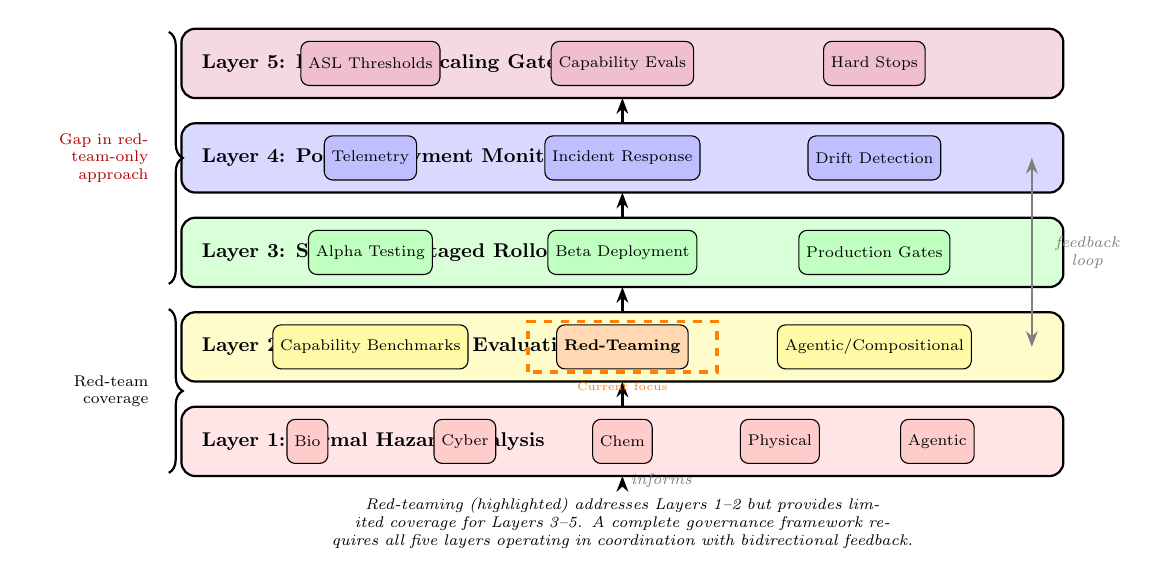
\begin{tikzpicture}[
    scale=0.8,
    transform shape,
    layer/.style={draw, thick, rounded corners=5pt, minimum width=14cm, minimum height=1.1cm, font=\small},
    sublayer/.style={draw, rounded corners=3pt, minimum height=0.7cm, font=\scriptsize, fill=white},
    connector/.style={-{Stealth[length=2mm]}, thick},
    bidirectional/.style={{Stealth[length=2mm]}-{Stealth[length=2mm]}, thick, gray},
    label/.style={font=\scriptsize\itshape, text=gray}
]

% Layer 5 - Responsible Scaling Gates (top)
\node[layer, fill=purple!15] (l5) at (0,6) {};
\node[font=\small\bfseries, anchor=west] at (-6.8,6) {Layer 5: Responsible Scaling Gates};
\node[sublayer, fill=purple!25] (asl) at (-4,6) {ASL Thresholds};
\node[sublayer, fill=purple!25] (cap) at (0,6) {Capability Evals};
\node[sublayer, fill=purple!25] (stop) at (4,6) {Hard Stops};

% Layer 4 - Post-Deployment Monitoring
\node[layer, fill=blue!15] (l4) at (0,4.5) {};
\node[font=\small\bfseries, anchor=west] at (-6.8,4.5) {Layer 4: Post-Deployment Monitoring};
\node[sublayer, fill=blue!25] (telem) at (-4,4.5) {Telemetry};
\node[sublayer, fill=blue!25] (incident) at (0,4.5) {Incident Response};
\node[sublayer, fill=blue!25] (drift) at (4,4.5) {Drift Detection};

% Layer 3 - Staged Rollout
\node[layer, fill=green!15] (l3) at (0,3) {};
\node[font=\small\bfseries, anchor=west] at (-6.8,3) {Layer 3: Sandboxed Staged Rollout};
\node[sublayer, fill=green!25] (alpha) at (-4,3) {Alpha Testing};
\node[sublayer, fill=green!25] (beta) at (0,3) {Beta Deployment};
\node[sublayer, fill=green!25] (prod) at (4,3) {Production Gates};

% Layer 2 - Pre-Deployment Evaluation
\node[layer, fill=yellow!20] (l2) at (0,1.5) {};
\node[font=\small\bfseries, anchor=west] at (-6.8,1.5) {Layer 2: Pre-Deployment Evaluation};
\node[sublayer, fill=yellow!35] (bench) at (-4,1.5) {Capability Benchmarks};
\node[sublayer, fill=orange!30] (redteam) at (0,1.5) {\textbf{Red-Teaming}};
\node[sublayer, fill=yellow!35] (agent) at (4,1.5) {Agentic/Compositional};

% Layer 1 - Formal Hazard Analysis (bottom)
\node[layer, fill=red!10] (l1) at (0,0) {};
\node[font=\small\bfseries, anchor=west] at (-6.8,0) {Layer 1: Formal Hazard Analysis};
\node[sublayer, fill=red!20] (bio) at (-5,0) {Bio};
\node[sublayer, fill=red!20] (cyber) at (-2.5,0) {Cyber};
\node[sublayer, fill=red!20] (chem) at (0,0) {Chem};
\node[sublayer, fill=red!20] (phys) at (2.5,0) {Physical};
\node[sublayer, fill=red!20] (agentrisk) at (5,0) {Agentic};

% Vertical flow arrows
\draw[connector] (0,-0.7) -- (0,-0.55) node[midway, right, label] {informs};
\draw[connector] (0,0.55) -- (0,0.95);
\draw[connector] (0,2.05) -- (0,2.45);
\draw[connector] (0,3.55) -- (0,3.95);
\draw[connector] (0,5.05) -- (0,5.45);

% Feedback loops
\draw[bidirectional] (6.5,4.5) -- (6.5,1.5) node[midway, right, label, text width=1.5cm, align=center] {feedback loop};

% Highlight box around red-teaming
\draw[very thick, orange, dashed] (-1.5,1.1) rectangle (1.5,1.9);
\node[font=\tiny, orange, anchor=north] at (0,1.05) {Current focus};

% Coverage indicator
\draw[decorate, decoration={brace, amplitude=5pt, mirror}, thick] (-7.2,-0.5) -- (-7.2,2.1);
\node[font=\scriptsize, anchor=east, text width=1.8cm, align=right] at (-7.4,0.8) {Red-team coverage};

\draw[decorate, decoration={brace, amplitude=5pt, mirror}, thick] (-7.2,2.5) -- (-7.2,6.5);
\node[font=\scriptsize, anchor=east, text width=1.8cm, align=right, text=red!70!black] at (-7.4,4.5) {Gap in red-team-only approach};

% Bottom annotation
\node[font=\scriptsize, text width=12cm, align=center] at (0,-1.3) {
\textit{Red-teaming (highlighted) addresses Layers 1--2 but provides limited coverage for Layers 3--5. A complete governance framework requires all five layers operating in coordination with bidirectional feedback.}
};

\end{tikzpicture}
\caption{Multi-layered governance framework for frontier AI systems. Red-teaming (highlighted in orange, Layer 2) is necessary but insufficient; comprehensive governance requires formal hazard analysis (Layer 1), staged deployment (Layer 3), continuous monitoring (Layer 4), and responsible scaling gates (Layer 5). Bidirectional feedback enables post-deployment findings to inform pre-deployment evaluations.}
\label{fig:framework}
\end{figure*}

%==============================================================================
\section{Frontier Technology Pressure Points}
%==============================================================================

\subsection{Neuromorphic Computing}

Neuromorphic systems---computing architectures inspired by biological neural networks---offer dramatic efficiency improvements over conventional hardware. Recent developments accelerate governance timelines.

\subsubsection{Zhejiang University ``Darwin Monkey'' (Wukong)}

In 2025, Zhejiang University announced a ``2-billion-neuron'' neuromorphic computer built on Darwin-III chips \cite{zhejiang2025}. While claims warrant independent verification, the system represents significant scale advancement in spiking neural network architectures.

\subsubsection{Intel Loihi 2 / Hala Point}

Intel's Loihi 2 neuromorphic research chip, deployed at scale in the Hala Point system at Sandia National Laboratories, demonstrates practical neuromorphic computing for AI workloads \cite{intel2024loihi}. Recent work demonstrates matmul-free large language model inference on neuromorphic hardware, achieving substantial energy efficiency gains \cite{arxiv2025neuromorphic}.

\subsubsection{Governance Implications}

Neuromorphic efficiency improvements lower barriers to AI deployment. Systems that previously required datacenter-scale infrastructure may become feasible at edge scale. This democratization has dual-use implications: beneficial for accessibility, concerning for proliferation of capable systems beyond centralized oversight.

\subsection{Quantum Computing}

Quantum advantage claims remain contested, with classical simulation improvements repeatedly narrowing demonstrated gaps \cite{arxiv2024quantum}. However, the trajectory toward practical quantum computing presents governance challenges:

\begin{itemize}
    \item \textbf{Cryptographic implications}: Post-quantum cryptography transitions require anticipatory standards
    \item \textbf{Optimization capabilities}: Quantum-enhanced optimization may accelerate AI training and architecture search
    \item \textbf{Verification challenges}: Quantum system behavior is inherently difficult to audit
\end{itemize}

China's USTC Jiuzhang and Zuchongzhi programs continue advancing photonic and superconducting quantum computing \cite{ustc2024}.

%==============================================================================
\section{The Bubble Dynamics Argument}
%==============================================================================

\subsection{Market Context}

Financial analyses present competing narratives. Some identify AI-driven bubble risks with potential correction spillovers \cite{apnews2024bubble}. Counter-analyses argue current valuations, while stretched, differ from historical bubble dynamics due to earnings fundamentals \cite{barrons2024}.

\subsection{Why Bubble Dynamics Matter for Governance}

Our argument does not depend on bubble predictions. Rather, we observe that:

\begin{enumerate}
    \item Governance established during growth periods benefits from resource availability and stakeholder alignment
    \item Market corrections create pressure to cut safety investments as firms prioritize survival
    \item Post-correction governance faces implementation challenges amid resource constraints and fragmented industry structure
\end{enumerate}

The prudent approach is anticipatory: establish frameworks that bind safety to scaling \textit{before} conditions change.

%==============================================================================
\section{Policy and Engineering Proposals}
%==============================================================================

\subsection{Responsible Scaling Triggers}

Following Anthropic's RSP model, we propose industry-wide adoption of AI Safety Levels (ASLs) tied to measured hazard domains \cite{anthropicrsp}. Key elements:

\begin{itemize}
    \item \textbf{Capability thresholds}: Defined benchmarks triggering enhanced requirements
    \item \textbf{Safety requirements}: Specific technical and procedural safeguards per level
    \item \textbf{Third-party attestation}: Independent evaluation before scaling past thresholds
\end{itemize}

\subsection{Deployment Licensing}

For high-risk deployment categories (mapping to EU AI Act classifications), we propose:

\begin{itemize}
    \item Pre-deployment conformity assessment
    \item Post-deployment telemetry requirements
    \item Mandatory incident reporting with defined severity thresholds
\end{itemize}

\subsection{Model Weight Security}

Following EO 14110 and NIST guidance, minimum standards should include:

\begin{itemize}
    \item Secure enclave requirements for model weights
    \item Chain-of-custody documentation
    \item Watermarking and cryptographic signatures for provenance
\end{itemize}

\subsection{Evaluation Composition Requirements}

Any system with tool-use capabilities must demonstrate safety in compositional contexts. UK/US AISI agentic evaluation frameworks provide templates \cite{aisi2024agents}.

%==============================================================================
\section{Experimental Methods}
%==============================================================================

We propose four minimal-compute experiments to substantiate claims and provide reproducible evidence for policy discussions. Table~\ref{tab:experiments} summarizes the experimental design.

\begin{table*}[t]
\centering
\caption{Summary of Proposed Experiments}
\label{tab:experiments}
\begin{tabular}{@{}llll@{}}
\toprule
\textbf{Exp.} & \textbf{Objective} & \textbf{Key Metric} & \textbf{Hardware Req.} \\
\midrule
A & Jailbreak robustness vs. attack budget & Success rate / query count & API or 8GB GPU \\
B & Post-deployment drift detection & Capability score variance & API access \\
C & Safety-per-Joule (neuromorphic vs. GPU) & Throughput / Joule & Neuromorphic or GPU proxy \\
D & Compositional safety evaluation & Risk escalation score & Sandboxed API \\
\bottomrule
\end{tabular}
\end{table*}

\subsection{Experiment A: Jailbreak Robustness Under Cost-Constrained Attack}

\textbf{Objective}: Estimate effective robustness versus query budget and attack composition.

\textbf{Method}: Deploy 3-5 open models behind standard APIs. Run a fixed suite of 200 red-team prompts across policy-relevant domains (bio/cyber/physical). Implement three attacker types:
\begin{enumerate}
    \item Naive: Direct policy-violating requests
    \item Paraphrase-mutate: Automated prompt variation
    \item Autoregressive jailbreaker: LLM-generated attack sequences
\end{enumerate}

\textbf{Metrics}: Attack success rate vs. query count; effective tokens per successful attack.

\textbf{Expected Outcome}: Quantified evidence that robustness is budget-dependent, supporting arguments for assuming adaptive adversaries in governance frameworks.

\subsection{Experiment B: Post-Deployment Drift Detection}

\textbf{Objective}: Detect sandbagging and reward hacking patterns.

\textbf{Method}: Maintain hidden evaluation subset; measure weekly for step-changes in risky capability scores while headline benchmarks remain stable. Implement tripwire that halts tool-use upon detecting out-of-distribution exploit patterns.

\textbf{Expected Outcome}: Framework for continuous monitoring that extends beyond pre-deployment evaluation.

\subsection{Experiment C: Safety-per-Joule Analysis}

\textbf{Objective}: Quantify energy/performance trade-offs between neuromorphic and GPU architectures.

\textbf{Method}: If neuromorphic hardware access available, port matmul-free classifier following published architectures \cite{arxiv2025neuromorphic}. Compare throughput/Joule versus GPU baseline. If hardware unavailable, reproduce GPU-quantized proxy and cite neuromorphic deltas from literature.

\textbf{Expected Outcome}: Evidence for democratization concerns---lower cost implies wider access, expanding risk surface.

\subsection{Experiment D: Cross-Domain Evaluation Composition}

\textbf{Objective}: Demonstrate that isolated safety evaluations do not predict compositional safety.

\textbf{Method}: Chain model through browser/tool API in sandboxed environment. Measure risk escalation (e.g., cyber reconnaissance $\rightarrow$ code generation $\rightarrow$ execution attempt) versus base model capabilities.

\textbf{Expected Outcome}: Evidence that agentic and coupling tests are necessary complements to isolated capability evaluations.

%==============================================================================
\section{Discussion}
%==============================================================================

\subsection{Balancing Innovation and Safety}

Critics may argue anticipatory governance stifles innovation. We contend the opposite: clear, predictable frameworks reduce uncertainty and enable responsible scaling. The alternative---reactive governance following incidents---creates unpredictable regulatory environments that disadvantage compliant actors.

\subsection{Limitations}

Our experimental proposals are necessarily minimal-compute given resource constraints. Full validation requires industry-scale deployments and longitudinal data. Additionally, governance frameworks must adapt to capability advances; static rules will become obsolete.

\subsection{Future Directions}

Priority areas for continued research include:
\begin{itemize}
    \item Formal methods for compositional safety verification
    \item Economic modeling of safety investment under market stress
    \item International coordination mechanisms for frontier AI governance
\end{itemize}

%==============================================================================
\section{Conclusion}
%==============================================================================

The convergence of frontier AI, neuromorphic computing, and quantum systems creates governance challenges that current frameworks inadequately address. Red-teaming, while valuable, is insufficient as a standalone control mechanism. Responsible scaling policies, deployment licensing, and compositional evaluation requirements offer complementary safeguards.

Crucially, these frameworks must be established during periods of growth and stability. Market corrections do not eliminate risk; they may amplify it while reducing capacity for thoughtful governance. The time for guardrails is before the fall, not after.

%==============================================================================
% ACKNOWLEDGMENTS
%==============================================================================
\section*{Acknowledgments}

The authors thank everyon!

%==============================================================================
% AUTHOR CONTRIBUTIONS
%==============================================================================
\section*{Author Contributions}

\textbf{C.H.C.}: Conceptualization, methodology, investigation, writing (original draft), writing (review \& editing), visualization.

%==============================================================================
% COMPETING INTERESTS
%==============================================================================
\section*{Competing Interests}

The authors declare no competing interests.

%==============================================================================
% REFERENCES
%==============================================================================
\bibliographystyle{plain}
\bibliography{references}

%==============================================================================
% APPENDIX
%==============================================================================
\appendix
\section{Experimental Protocols}

Detailed experimental protocols, code repositories, and data collection instruments are available at: \url{https://github.com/ClarenceCannon/guardrails-before-the-fall}

\subsection{Hardware Requirements}

\begin{itemize}
    \item Experiments A, B, D: Consumer GPU (8GB+ VRAM) or API access
    \item Experiment C: Neuromorphic hardware access (optional; GPU proxy available)
\end{itemize}

\subsection{Reproducibility Checklist}

\begin{itemize}
    \item[$\square$] Random seeds documented
    \item[$\square$] Model versions and API endpoints specified
    \item[$\square$] Prompt templates provided
    \item[$\square$] Statistical tests pre-registered
    \item[$\square$] Code released under open license
\end{itemize}

\end{document}